\documentclass[a4paper,abstracton]{scrreprt}
\usepackage[T1]{fontenc}
\usepackage[utf8]{inputenc}
\usepackage[ngerman]{babel}
\usepackage{pdfpages} 

%correct linebreaking in bibliography
\usepackage{hyperref}
\usepackage{breakurl}

%Formatierung des Inhaltsverzeichnisses
\usepackage{tocloft}
\cftsetindents{chapter}{0in}{0.5in}
\cftsetindents{section}{0in}{0.5in}
\cftsetindents{subsection}{0in}{0.5in}
\setlength\cftbeforechapskip{18pt}


%pictures
\usepackage{float}
\usepackage{graphicx}
\graphicspath{{img/}}

%biblatex
\usepackage[babel,german=quotes]{csquotes}
\usepackage[style=authortitle]{biblatex}

\bibliography{literatur}
\defbibheading{lit}{\chapter{Literaturverzeichnis}}
\setlength\bibitemsep{2\itemsep}

\usepackage{filecontents}
\begin{filecontents}{literatur.bib} 
@Electronic{faktenuber,
  Title                    = {Fakten über Seitlinge},
  Author                   = {fakten-uber.de},
  Url                      = {http://fakten-uber.de/seitlinge},
  Keywords                 = {faktenuber},
  Note                     = {Navigation: Suche, Seitlinge},
  Owner                    = {Benedikt},
  Urldate				   = {2014-07-05}
}
@Electronic{pilzech,
	Title					= {Pilzbestimmung Pleurotus},
	Author					= {www.pilze.ch},
	Url						= {http://www.pilze.ch/pilzbestimmung/artenlisten/Pleurotus.htm},
	Keywords				= {pilze.ch},
	Note					= {Navigation: Pilzbestimmung, Gattungen und Arten, Pleurotus},
	Urldate					= {2014-07-05}
}
@Electronic{pg_austernseitling,
	Title					= {Pilzgalerie Austernseitling},
	Author					= {www.123pilze.de},
	Url						= {http://www.123pilze.de/DreamHC/Download/Austernseitling1105.htm},
	Keywords				= {www.123pilze.de},
	Note					= {Navigation: Pilze nach Alphabet geordnet, Austernseitling},
	Urldate					= {2014-07-05}
}
@Electronic{vital,
	Title					= {Vitalpilzratgeber},
	Author					= {www.vitalpilzratgeber.de},
	Url						= {http://www.vitalpilzratgeber.de/pleurotus/},
	Keywords				= {www.vitalpilzratgeber.de},
	Note					= {Navigation: Pleurotus},
	Urldate					= {2014-07-05}
}
@Electronic{pg_ohrfoermig,
	Title					=  {Pilzgalerie Ohrförmiger Seitling},
	Author					= {www.123pilze.de},
	Url						= {http://www.123pilze.de/DreamHC/Download/OhrfoermigerSeitling.htm},
	Keywords				= {www.123pilze.de},
	Note					= {Navigation: Pilze nach Alphabet geordnet, Ohrförmiger Seitling},
	Urldate					= {2014-07-06}
}
@Online{deutschlandradio,
	Title					=  {Speisepilz wird Giftpilz},
	Author					= {Udo Pollmer},
	month = jun,
	year = {2008},
	Url						= {http://www.deutschlandradiokultur.de/speisepilz-wird-giftpilz.993.de.html?dram:article_id=154417},
	Keywords				= {www.deutschlandradiokultur.de},
	Note					= {Navigation: Suche nach \emph{Speisepilz wird Giftpilz}, Ohrförmiger Seitling},
	Urldate					= {2014-07-06}
}
@Electronic{tintling_auster,
	Title					=  {Austernseitling \emph{Pleurotus ostreatus}},
	Author					= {www.tintling.com},
	Url						= {http://tintling.com/pilzbuch/arten/p/Pleurotus_ostreatus.html},
	Keywords				= {www.tintling.com},
	Note					= {Navigation: Pilzbuch, Gattungen, Pleurotus,  Pleurotus ostreatus},
	Urldate					= {2014-07-06}
}
@online{pilzfinder_austernseitling_image,
	Title					= {Austernseitling},
	Author					= {Jürgen Mathes},
	Url						= {http://www.pilzfinder.de/highlight/auster2.jpg},
	Keywords				= {www.pilzfinder.de},
	Note					= {Navigation: Pilze von A -- Z, Austernseitling, oberstes Bild},
	month = jan,
	year = {2012},
	day = {1},
	Urldate					= {2014-07-06}
}
\end{filecontents} 

%set numeration depth
\setcounter{secnumdepth}{3}
%set how many numbers show up in table-of-contents
\setcounter{tocdepth}{2}

\begin{document}
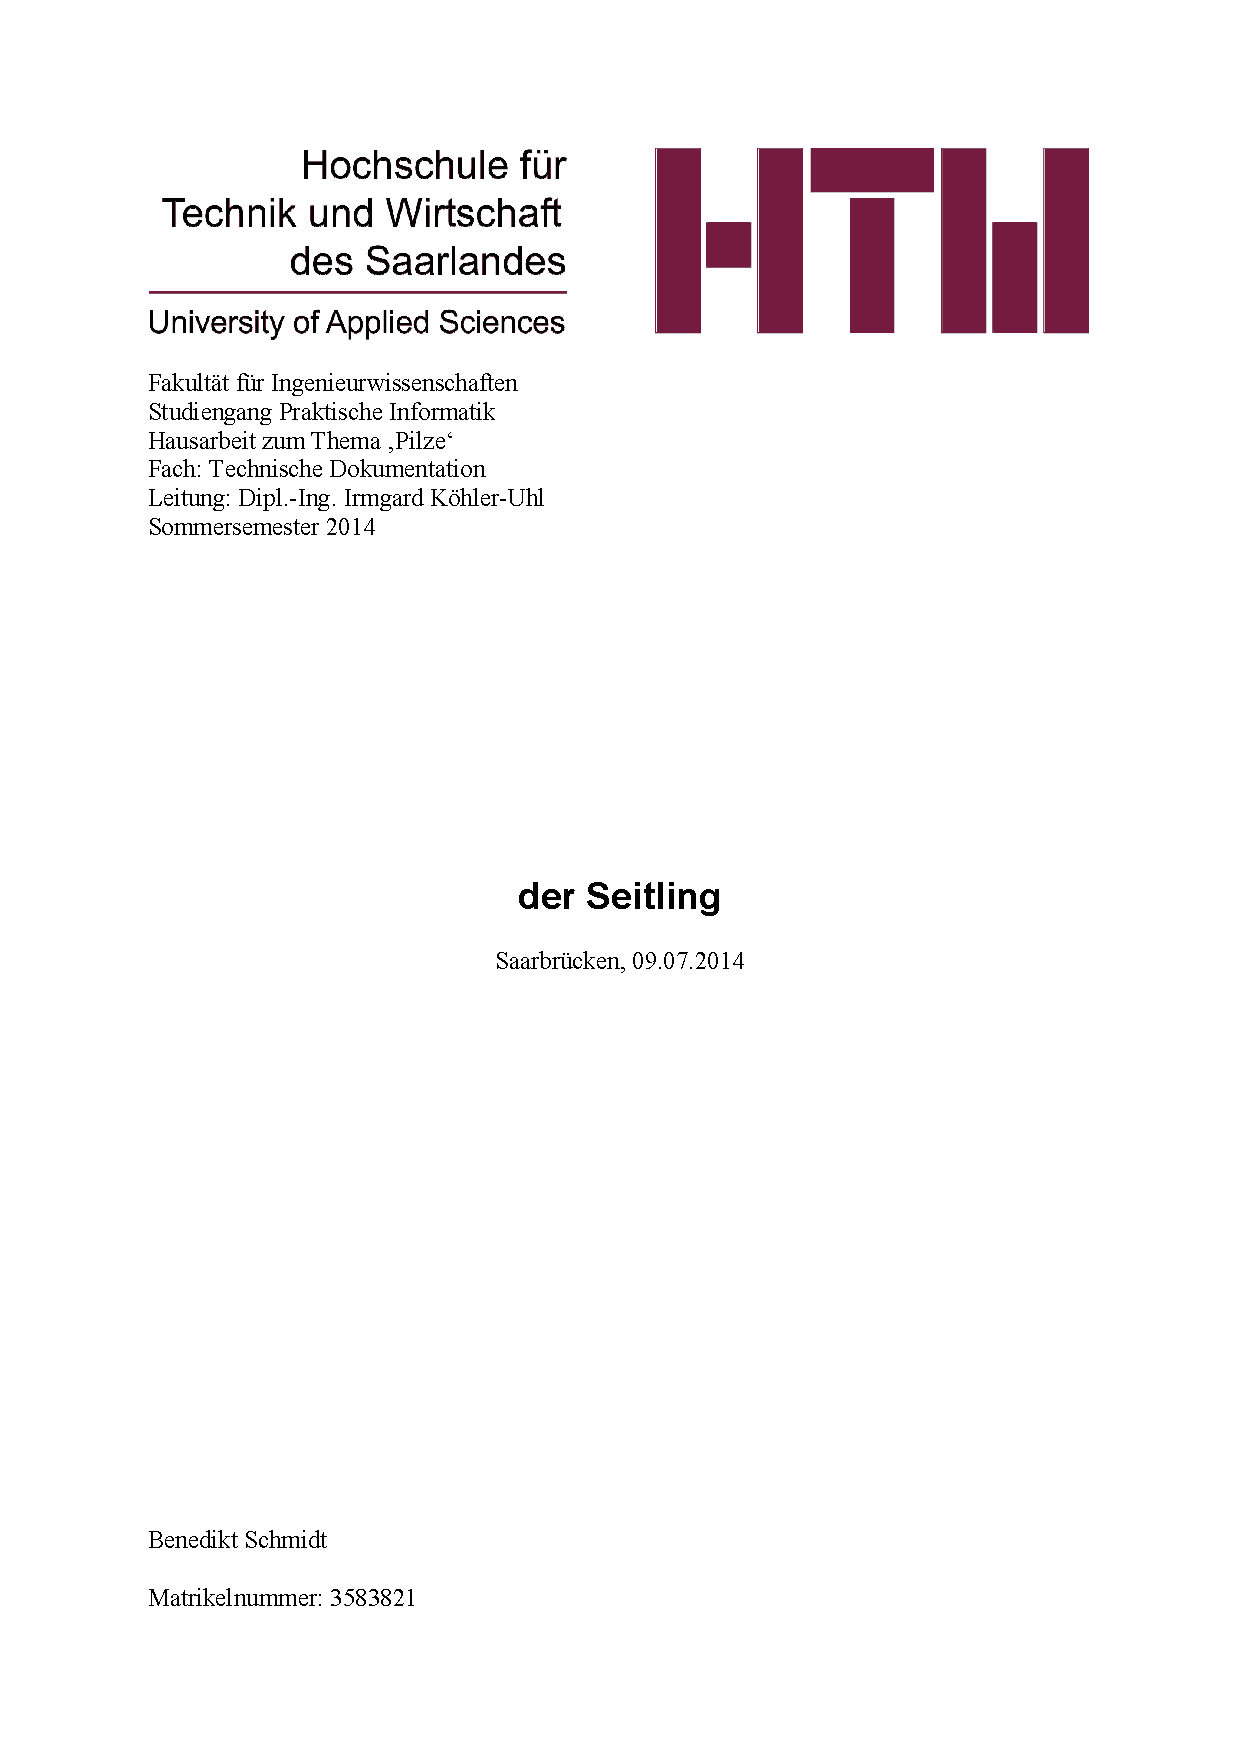
\includepdf[]{Deckblatt_Seitling.pdf}

%\author{Benedikt Schmidt}
%\subject{Pilze}
%\title{der Seitling}
%\publishers{htwsaar}
%\maketitle
\tableofcontents
\pagebreak
\listoffigures
%\listoftables

\begin{abstract}
\begin{quote}%abstand rechts und links
Unter dem Schirmthema \emph{Heimische Pilze} beschäftigt sich diese Ausarbeitung mit den Seitlingen (lat.: "'Pleurotus"'). Es werden unter anderem Kenntnisse über Allgemeinheiten, das Vorkommen, die Beschreibung des Pilzes sowie die bei Pilzen so wichtigen Verwechslungsmöglichkeiten vermittelt. Weiterhin wird eine Auswahl ausgesuchter Arten einzeln betrachtet.
\end{quote} 
\end{abstract}

\chapter{Vorwort}
Diese Ausarbeitung ist Bestandteil einer Reihe von Ausarbeitungen, die im Zuge der Vorlesung "'Technische Dokumentation"' entstanden sind. Der Kerngedanke bei der Anfertigung dieser Arbeit ist, zu erlernen, wie man mit fachbezogenen Texten umgeht -- von der Recherche über die Erstellung bis hin zur Anfertigung eines korrekten Literaturverzeichnisses. 

\chapter{Der Seitling}
\section{Allgemeines}
Die Seitlinge (lat. \emph{Pleurotus}) sind eine Pilzgattung aus der Familie der Seitlingsverwandten. In der Vergangenheit wurde sie lange den Stielporlingsverwandten (Polyporaceae) zugerechnet. Der lateinische Name \emph{Pleurotus} leitet sich von griechisch \emph{pleura} = die Seite, und griechisch \emph{us} = das Ohr ab, da die Pilze oft ohrförmig sind und meist einen seitlichen Stiel besitzen.\footcite{faktenuber} 

\section{Vorkommen}
Da Seitlinge eine große Gattung darstellen, wachsen diese auch an unterschiedlichsten Orten und unter verschiedenen Bedingungen. Sie sind auch nicht unbedingt zu einer ganz speziellen Jahreszeit anzutreffen. Viele Arten wachsen vorrangig zwischen Sommer und Herbst, einige sind jedoch auch im Winter zu sichten, wie zum Beispiel der Gemeine Orangenseitling (lat. \emph{Phyllotopsis nidulans}). Andere Arten wachsen bereits im Frühjahr, wie zum Beispiel der Lungenseitling (lat. \emph{Pleurotus pulmonarius})

Seitlinge wachsen meist auf Holz, teilweise aber auch auf Erde, Stroh oder toten Blättern. Dabei sind sie hauptsächlich auf totem Laub- oder Nadelholz, bzw. an morschem Bauholz anzutreffen.\footcite{pilzech}

\section{Beschreibung}
Bei den Seitlingen handelt es sich meist um seitlich wachsende Pilze mit kurzem beziehungsweise ohne Stiel. Ihre Hüte sind muschel-, nieren- oder halbkreisförmig. Die Hutunterseite wird durch helle, ganzrandige Lamellen gebildet. Sie laufen dem Stiel entlang herab. Die Hutoberseite hingegen ist kahl und nicht geschuppt. Sie ist ockerlich bis grau, graublau, grünlichgrau und glatt. Das Sporenpulver ist weiß und in seltenen Fällen etwas lila. Das Fleisch der Seitlinge hat bei jungen Fruchtkörpern eine saftige, alt balt eine zähle Konsistenz.\footcite{faktenuber}\footcite{pilzech}\\
Die meisten Seitlinge sind nicht für den Verzehr geeignet. Einige Pilze, wie zum Beispiel der Austernseitling (lat. \emph{Pleurotus ostreatus}) sind jedoch als Speisepilze anerkannt.\footcite{pg_austernseitling}

\section{Arten}
"'Die Gattung Pleurotus umfasst weltweit etwa 30 Arten. In Europa kommen 8 Arten vor bzw. sind dort zu erwarten."' \footcite{faktenuber} Im folgenden sollen die bekanntesten Vertreter der Gattung kurz beschrieben werden.

\subsection{Austernseitling}
Der im Durchmesser 5 bis 20 cm große Austernseitling ist der wohl bekannteste Vertreter der Seitlinge. Der Speisepilz kommt vorzugsweise an Rotbuchen vor, aber auch an vielen anderen Bäumen und sogar auf Stroh. In Mitteleuropa ist er recht häufig anzutreffen. Seine Hüte sind muschelförmig, meistens ohne deutlich abgesetzten Stiel. Seine Oberfläche ist glatt, feucht und fett glänzend, seine Farbe reicht von schiefergrau über blaugrau bis graubraun. Die Lamellen sind weiß, dünn und engstehend. Sein Fleisch ist dick, fest und im Sielt zäh.

Im Vergleich zu anderen Pilzarten ist der Austernseitling auch unter winterlichen Bedingungen noch zu finden. Er ist einer der bei uns am häufigsten angebotenen Kulturspeisepilze. Sein Geruch und Geschmack sind pilzartig-aromatisch.\footcite{tintling_auster}

\begin{figure}[H]
\centering
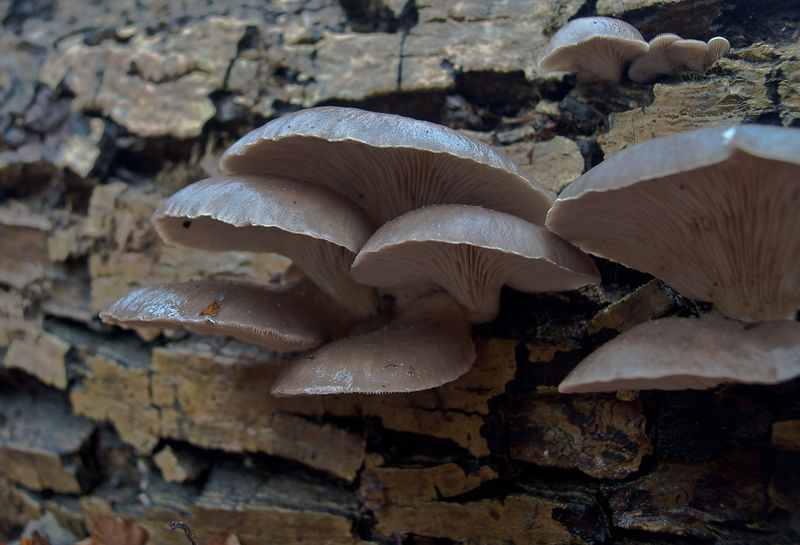
\includegraphics[scale=0.6]{auster2}
\caption{der Austernseitling\protect\footnotemark}
\label{fig:austernseitling}
\end{figure}
\footnotetext{\cite{pilzfinder_austernseitling_image}}

\section{Medizinische Bedeutung}
Durch die in manchen Seitlingen vorhandene, antibiotisch wirkende Subtanz \emph{Pleuromulin} werden die Pilze unter anderem in der Traditionellen Chinesischen Medizin eingesetzt, zum Beispiel bei der Behandlung von Hexenschüssen und hohen Cholesterinwerten. Ebenfalls sind verschiedene Vitamine des Vitamin-B-Komplexes enthalten, die im menschlichen Organismus zur Energiegewinnung notwendig sind. Da diese Vitamine normalerweise über den Verzehr von Fleischprodukten aufgenommen werden, bieten die Seitlinge eine gute Alternative, wenn der Fleischverzehr aus ethischen oder moralischen Gründen nicht möglich ist. 

Daneben gibt es noch weitere Einsatzmöglichkeiten im Bereich der Entzündungshemmung, Aufnahme von Ballaststoffen, Blutdrucksenkung und Krebsheilung.
Vor allem sind dabei die beiden Arten Austernseitling und Kräuterseitling zu nennen.\footcite{vital} Es ist jedoch anzumerken, dass nicht alle Seitlinge für die medizinische Verwendung geeignet sind.

\section{Verwechslungsmöglichkeiten}
Die Verwechslungsgefahr der Seitlinge ist vor allem zu anderen Seitlingen relativ hoch. Dadurch, dass einige Seitlingsarten essbar, andere jedoch giftig sind, ist hier äußerste Vorsicht geboten. Gerade der Ohrförmige Seitling kann zum Beispiel mit dem Speisepilz Lungenseitling (lat. \emph{Pleurotus pulmonaris}) verwechselt werden. Wer diesen nicht zu 100\% identifizieren kann, sollte ihn besser meiden und nicht verzehren, da dies unter Umständen tödliche Folgen mit sich bringen kann.\footcite{pg_ohrfoermig}\footcite{deutschlandradio}

\section{Ernte, Haltbarkeit und richtige Lagerung}

\section{Rezept}

\printbibliography[heading=lit]

\end{document}
